\documentclass[10pt,landscape,letterpaper]{article}
\usepackage[utf8]{inputenc}
\usepackage[T1]{fontenc}
\usepackage{lmodern}
%\usepackage[LY1,T1]{fontenc}
%\usepackage{frutigernext}
%\usepackage[lf,minionint]{MinionPro}
\usepackage{tikz}
\usetikzlibrary{automata,shapes,positioning,arrows,fit,calc,graphs,graphs.standard}
\usepackage[nosf]{kpfonts}
\usepackage[t1]{sourcesanspro}
\usepackage{multicol}
\usepackage{wrapfig}
\usepackage[top=6mm,bottom=6mm,left=6mm,right=6mm]{geometry}
\usepackage[framemethod=tikz]{mdframed}
\usepackage{microtype}
\usepackage{pdfpages}
\usepackage[]{minted}
\usepackage{lipsum}
% https://tex.stackexchange.com/a/112573
\usepackage[most]{tcolorbox}
\usepackage{etoolbox}
\usepackage{listings}
\usepackage{realboxes}
\usetikzlibrary{arrows.meta}
\usepackage{enumitem} % allow to change list item separation
\usepackage{multirow}

% for easy SI units
\usepackage{siunitx}

\let\bar\overline

\definecolor{myblue}{cmyk}{1,.72,0,.38}

\def\firstcircle{(0,0) circle (1.5cm)}
\def\secondcircle{(0:2cm) circle (1.5cm)}

\colorlet{circle edge}{myblue}
\colorlet{circle area}{myblue!5}

\tikzset{filled/.style={fill=circle area, draw=circle edge, thick},
    outline/.style={draw=circle edge, thick}}
    
\pgfdeclarelayer{background}
\pgfsetlayers{background,main}

\everymath\expandafter{\the\everymath \color{myblue}}
\everydisplay\expandafter{\the\everydisplay \color{myblue}}

\renewcommand{\baselinestretch}{.8}
\pagestyle{empty}

\global\mdfdefinestyle{header}{%
linecolor=gray,linewidth=1pt,%
leftmargin=0mm,rightmargin=0mm,skipbelow=0mm,skipabove=0mm,
}

\newcommand{\header}{
\begin{mdframed}[style=header]
\footnotesize
\sffamily
Hilfszettel zur Klausur\\
von~Tim~S.,~Seite~\thepage~von~2
\end{mdframed}
}

% more compact minted custom frames
\newtcolorbox{mintedbox}[1][]
{
  colframe = black!20,
  colback  = white,
  left = 0pt,
  right = 0pt,
  top = 0pt,
  bottom = 0pt,
  #1,
}

% make code font smaller
\setminted{fontsize=\footnotesize}

% nicer frame for minted environments
\BeforeBeginEnvironment{minted}{\begin{mintedbox}}%
\AfterEndEnvironment{minted}{\end{mintedbox}}%


\makeatletter % Author: https://tex.stackexchange.com/questions/218587/how-to-set-one-header-for-each-page-using-multicols
\renewcommand{\section}{\@startsection{section}{1}{0mm}%
                                {.2ex}%
                                {.2ex}%x
                                {\color{myblue}\sffamily\normalsize\bfseries}}
\renewcommand{\subsection}{\@startsection{subsection}{1}{0mm}%
                                {.2ex}%
                                {.2ex}%x
                                {\sffamily\bfseries}}



% \def\multi@column@out{%
%    \ifnum\outputpenalty <-\@M
%    \speci@ls \else
%    \ifvoid\colbreak@box\else
%      \mult@info\@ne{Re-adding forced
%                break(s) for splitting}%
%      \setbox\@cclv\vbox{%
%         \unvbox\colbreak@box
%         \penalty-\@Mv\unvbox\@cclv}%
%    \fi
%    \splittopskip\topskip
%    \splitmaxdepth\maxdepth
%    \dimen@\@colroom
%    \divide\skip\footins\col@number
%    \ifvoid\footins \else
%       \leave@mult@footins
%    \fi
%    \let\ifshr@kingsaved\ifshr@king
%    \ifvbox \@kludgeins
%      \advance \dimen@ -\ht\@kludgeins
%      \ifdim \wd\@kludgeins>\z@
%         \shr@nkingtrue
%      \fi
%    \fi
%    \process@cols\mult@gfirstbox{%
% %%%%% START CHANGE
% \ifnum\count@=\numexpr\mult@rightbox+2\relax
%           \setbox\count@\vsplit\@cclv to \dimexpr \dimen@-1cm\relax
% \setbox\count@\vbox to \dimen@{\vbox to 1cm{\header}\unvbox\count@\vss}%
% \else
%       \setbox\count@\vsplit\@cclv to \dimen@
% \fi
% %%%%% END CHANGE
%             \set@keptmarks
%             \setbox\count@
%                  \vbox to\dimen@
%                   {\unvbox\count@
%                    \remove@discardable@items
%                    \ifshr@nking\vfill\fi}%
%            }%
%    \setbox\mult@rightbox
%        \vsplit\@cclv to\dimen@
%    \set@keptmarks
%    \setbox\mult@rightbox\vbox to\dimen@
%           {\unvbox\mult@rightbox
%            \remove@discardable@items
%            \ifshr@nking\vfill\fi}%
%    \let\ifshr@king\ifshr@kingsaved
%    \ifvoid\@cclv \else
%        \unvbox\@cclv
%        \ifnum\outputpenalty=\@M
%        \else
%           \penalty\outputpenalty
%        \fi
%        \ifvoid\footins\else
%          \PackageWarning{multicol}%
%           {I moved some lines to
%            the next page.\MessageBreak
%            Footnotes on page
%            \thepage\space might be wrong}%
%        \fi
%        \ifnum \c@tracingmulticols>\thr@@
%                     \hrule\allowbreak \fi
%    \fi
%    \ifx\@empty\kept@firstmark
%       \let\firstmark\kept@topmark
%       \let\botmark\kept@topmark
%    \else
%       \let\firstmark\kept@firstmark
%       \let\botmark\kept@botmark
%    \fi
%    \let\topmark\kept@topmark
%    \mult@info\tw@
%         {Use kept top mark:\MessageBreak
%           \meaning\kept@topmark
%          \MessageBreak
%          Use kept first mark:\MessageBreak
%           \meaning\kept@firstmark
%         \MessageBreak
%          Use kept bot mark:\MessageBreak
%           \meaning\kept@botmark
%         \MessageBreak
%          Produce first mark:\MessageBreak
%           \meaning\firstmark
%         \MessageBreak
%         Produce bot mark:\MessageBreak
%           \meaning\botmark
%          \@gobbletwo}%
%    \setbox\@cclv\vbox{\unvbox\partial@page
%                       \page@sofar}%
%    \@makecol\@outputpage
%      \global\let\kept@topmark\botmark
%      \global\let\kept@firstmark\@empty
%      \global\let\kept@botmark\@empty
%      \mult@info\tw@
%         {(Re)Init top mark:\MessageBreak
%          \meaning\kept@topmark
%          \@gobbletwo}%
%    \global\@colroom\@colht
%    \global \@mparbottom \z@
%    \process@deferreds
%    \@whilesw\if@fcolmade\fi{\@outputpage
%       \global\@colroom\@colht
%       \process@deferreds}%
%    \mult@info\@ne
%      {Colroom:\MessageBreak
%       \the\@colht\space
%               after float space removed
%               = \the\@colroom \@gobble}%
%     \set@mult@vsize \global
%   \fi}

\makeatother
\setlength{\parindent}{0pt}

\begin{document}
%\footnotesize
\small
\begin{multicols*}{5}
  \section{Homework Examples}
\subsection*{Delay (tabulation)}
\begin{center}
  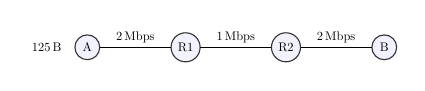
\begin{tikzpicture}[
    scale = 0.45, transform shape,
    >={Latex[black, length=1mm]},
    node distance=2cm,
    roundnode/.style={
        circle, draw=black!80, fill=blue!5, minimum size=7mm
      },
  ]
  \node[roundnode](A) {A};
  \node[roundnode](R1) [right=of A] {R1};
  \node[roundnode](R2) [right=of R1] {R2};
  \node[roundnode](B) [right=of R2] {B};
  \node[node distance=0.25cm] [left=of A] {\qty{125}{\byte}};
  \path[-]
    (A) edge [] node[above]{\qty{2}{Mbps}} (R1)
    (R1) edge [] node[above]{\qty{1}{Mbps}} (R2)
    (R2) edge [] node[above]{\qty{2}{Mbps}} (B)
  ;
  \end{tikzpicture}
  \begin{scriptsize}
    \begin{itemize}
      \item sending 4 packets from A to B
      \item propagation delay is \qty{5}{\milli\second} for all links
    \end{itemize}
  \end{scriptsize}
  \resizebox{5cm}{!}{
    \begin{tabular}{ |r|r|r|r|r|r|r| }
      \hline
      \multicolumn{1}{|c|}{P$_{\#}$} & \multicolumn{1}{c|}{A$\to$} & \multicolumn{1}{c|}{$\to$R1} & \multicolumn{1}{c|}{R1$\to$} & \multicolumn{1}{c|}{$\to$R2} & \multicolumn{1}{c|}{R2$\to$} & \multicolumn{1}{c|}{$\to$B} \\ [0.6ex]
      \hline
      1 & 0.5ms & 5.5ms & 6.5ms & 11.5ms & 12ms & 17ms \\
      \hline
      2 & 1ms & 6ms & 7.5ms & 12.5ms & 13ms & 18ms \\
      \hline
      3 & 1.5ms & 6.5ms & 8.5ms & 13.5ms & 14ms & 19ms \\
      \hline
      4 & 2ms & 7ms & 9.5ms & 14.5ms & 15ms & 20ms \\
      \hline
    \end{tabular}
  }
\end{center}
  \section{Quick Facts}
\subsection*{Miscellaneous Tips}
\footnotesize
\blockquote{A DNS server using UDP will query a different authoritative
server if its first query is lost (assuming there are multiple
authoritative servers). It attempts to maximize hit probability.}

\blockquote{A TCP handshake takes 1 RTT}

\blockquote{\textbf{Fast retransmission} requires 3 packets losses to be
triggered, and it halves the cwnd. \textbf{Slow retransmission} waits
for the recovery timer to expire and resets the cwnd}

\blockquote{\textbf{Stub resolver} must know the IP address of a caching
resolver. These are usually are the end users.}

\blockquote{\textbf{Cache resolvers} must know the IP address of a root
server.}

\blockquote{\textbf{Authoritative server} the final source of truth
(either address or CNAME).}

\small
\subsection*{Internet Protocol Stack}
\begin{itemize}
  \item \textbf{application}: DNS, FTP, SMTP, HTTP
  \item \textbf{transport}: TCP, UDP
  \item \textbf{network}: IP
  \item \textbf{link}: ethernet, WiFi
\end{itemize}
\subsection*{Stateless Protocols}
\begin{itemize}
  \item HTTP/1.1
  \item DNS
  \item UDP
\end{itemize}
\subsection*{Stateful Protocols}
\begin{itemize}
  \item TCP
\end{itemize}
\subsection*{Has re-trans. timers}
\begin{itemize}
  \item DNS caching resolver
  \item TCP data sender
\end{itemize}
\subsection*{DOESN'T have re-trans. Timers}
\begin{itemize}
  \item HTTP client/server
  \item DNS auth. server
  \item TCP data receiver
\end{itemize}
\subsection*{Common HTTP responses}
\begin{itemize}
  \item 200 OK: request succeeded
  \item 301 Moved Permanently: object moved to a location specified in the message
  \item 400 bad request: message not understood by server
  \item 505 HTTP version not supported
\end{itemize}
\subsection*{HTTP/1.0}
It uses TCP. Allows 1 request per connection. Each request needs to
reopen a connection. Allows parallel connections. Does not allow
pipelining
\subsection*{HTTP/1.1}
It uses TCP. Connection is persistent. As many requests per connection.
Allows pipelining and parallel connections.
\subsection*{HTTP/2.0}
Similar to HTTP/1.1 but it brakes down large packets into frames. This
allows to prevent some forms of head-of-line blocking (cannot prevent
inherent TCP HoL blocking). It also allows to send multiple streams of
data for multiplexing.
\subsection*{HTTP Packet Types}
\resizebox{5cm}{!}{
  \begin{tabular}{ |l|l|l|l|l|l|l| }
    \hline
    \multicolumn{1}{|c|}{Type} & \multicolumn{1}{|c|}{HTTP/1.0} & \multicolumn{1}{|c|}{HTTP/1.1} \\
    \hline
    GET    & yes      & yes \\
    \hline
    POST   & yes      & yes \\
    \hline
    HEAD   & yes      & yes \\
    \hline
    PUT    & no       & yes \\
    \hline
    DELETE & no       & yes \\
    \hline
  \end{tabular}
}
\subsection*{TCP + TLS}
\begin{center}
  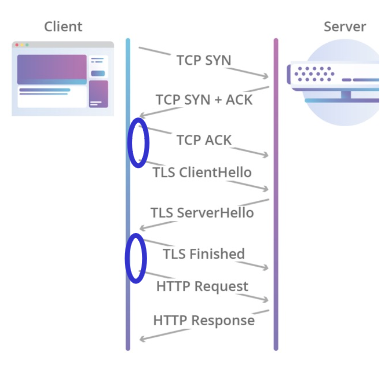
\includegraphics[scale=0.4]{images/tcp-n-tls.png}
\end{center}
\subsection*{Go-Back-N}
Sender has sliding window and can send many unacknowledged packets.
Acknowledgement is for the latest received packet w/o error and sender
window slides. On packet loss it retransmits all packets in the sliding
window. ACKs are cumulative. It does not buffers packets.
\subsection*{Selective Repeat}
Sender has sliding window and can send many unacknowledged packets.
Receiver acknowledges each received packet, and it buffers them
(out-of-order if necessary). Sender "selects" ACKed packets and re-sends
unACKed ones when their individual timers expire.
  \section{Formulae}
\subsection{ratios}
\begin{scriptsize}
P/E Ratio = Price Per Share / Earnings Per Share \\
Market to Book Ratio = Market Value per Share / Book Value per Share \\
Current Ratio = Current Assets/ Current Liabilities \\
Quick Ratio = (Current Assets - Inventory) / Current Liabilities \\
Cash Ratio = Cash / Current Liabilities \\
Debt/Equity = Total Debt / Total Equities \\
Total Debt Ratio = (Total Assets - Total Equity ) / Total Assets \\
Dividend Payout Ratio = Dividends / Net Income \\
Retention Ratio = (Net Income - Dividends) / Net Income \\
\end{scriptsize}
\subsection{others}
\begin{scriptsize}
Market Capitalization = Price per share $\times$ \# Shares Outstanding \\
Equity Multiplier = Total Assets / Total Equity \\
Times Interest Earned = (Earnings Before Interest And Taxes) / Interest \\
Cash Coverage = (EBIT + Depreciation + Amortization) / Interest \\
Inventory Turnover = Cost of Goods Sold / Inventory \\
Days' Sales in Inventory = 365 / (Inventory Turnover) \\
Receivables Turnover = Sales / Accounts Receivable \\
Days' Sales in Receivables = 365 / Receivables Turnover \\
Total Asset Turnover = Sales  /Total Assets  \\
Profit Margin = Net Income / Sales \\
\textbf{R}eturn \textbf{o}n \textbf{A}ssets = Net Income / Total Assets \\
\textbf{R}eturn \textbf{o}n \textbf{E}quity = Net Income / Total Equity \\
EBITDA Margin = EBITDA / Sales \\
Capital Intensity = Total Assets / Sales \\
\end{scriptsize}
\subsection{EFN (external financing need)}
Where \\
$\mathrm{AS} = \frac{\mathrm{Assets}}{\mathrm{Sales}}\times\Delta\mathrm{Sales}$ \\
$\mathrm{LS} = \frac{\text{Spon. Liab.}}{\mathrm{Sales}}\times\Delta\mathrm{Sales}$ \\
$\Delta\mathrm{Earnings} = \text{Profit Margin}\times\text{Proj. Sales}\times\left(1 - d\right)$ \\
Then \\
$\mathrm{EFN} = \mathrm{AS} - \mathrm{LS} - \Delta\mathrm{Earnings}$ \\
$d = \text{dividend payout ratio}$ \\
$b = (1 - d) = \text{retention ratio}$ \\

\subsection{Internal Growth Rate}
$\mathrm{IGR} = \frac{\mathrm{ROA}\times b}{1-\mathrm{ROA}\times b}$
\subsection{Sustainable Growth Rate}
$\mathrm{SGR} = \frac{\mathrm{ROE}\times b}{1-\mathrm{ROE}\times b}$
\subsection{Net Present Value}
$\mathrm{NVP} = \sum_{n=0}^T~\text{CF}_n/(1+r)^n$
\subsection{Annuity}
$\mathrm{PV} = (A/r)(1-(1+r)^{-n})$
\subsection{Holding Period Return}
This is the return that an investor would get when holding an investment over a period of years.
$\mathrm{HPR} = (1+R_1)\times(1+R_2)\times\dots\times(1+R_T) - 1$
\subsection{Geometric Return}
$\mathrm{R_g} = \sqrt[T]{(1+R_1)\times(1+R_2)\times\dots\times(1+R_T)} - 1$
\subsection{Arithmetic Return}
$\mathrm{R_g} = \frac{(1+R_1)+(1+R_2)+\dots+(1+R_T)}{T}$
  \section{Terminology}
name server (NS), resource record (RR), content distribution network
(CDN), top level domains (TLDs), canonical name (CNAME), address (A),
transmission control protocol (TCP), user datagram protocol (UDP),
internet protocol (IP), maximum transmit unit (MTU), Don't fragment bit
(DF bit), More fragments bit (MF bit), Classless Inter-Domain Routing
(CIDR), Netowrk address translation (NAT), Message Authenticatio Code
(MAC in cryptography), Hash based MAC (HMAC), Medium Access Control (MAC
in networking), Open Shortest Path First (OSPF), Border Gateway Protocol
(BGP), autonomous systems (AS)
\end{multicols*}
\newpage
\begin{multicols*}{3}
  \section{Tables \& Diagrams}
\subsection{Congestion Control FSM}
\begingroup
\renewcommand{\arraystretch}{1.5} % Default value: 1
\begin{center}
  \resizebox{8cm}{!}{
    \begin{tabular}{|l|l|l|}
      \hline
      \multicolumn{3}{|c|}{\Large{Slow Start}}                                                     \\
      \hline
      Event Trigger                & Transition to                  & Action(s)                    \\
      \hline
      \hline
      \multirow{3}{*}{new ACK}     & \multirow{3}{*}{loop back}     & cwnd $\to$ cwnd + MSS        \\
      ~                            & ~                              & dupACK $\to$ 0               \\
      ~                            & ~                              & transmit new segments        \\
      \hline
      dupe ACK                     & loop back                      & dupACK++                     \\
      \hline
      cwnd $\geq$ ssthresh         & Congestion Avoidance           & do nothing                   \\
      \hline
      \multirow{4}{*}{timeout}     & \multirow{4}{*}{loop back}     & ssthresh $\to$ cwnd / 2      \\
      ~                            & ~                              & cwnd $\to$ 1 MSS             \\
      ~                            & ~                              & dupACK $\to$ 0               \\
      ~                            & ~                              & re-transmit missing segments \\
      \hline
      \multirow{3}{*}{dupACK == 3} & \multirow{3}{*}{Fast Recovery} & ssthresh $\to$ cwnd / 2      \\
      ~                            & ~                              & cwnd $\to$ ssthresh + 3 MSS  \\
      ~                            & ~                              & re-transmit missing segments \\
      \hline
    \end{tabular}
  }
\end{center}%
\begin{center}
  \resizebox{8cm}{!}{
    \begin{tabular}{|l|l|l|}
      \hline
      \multicolumn{3}{|c|}{\Large{Congestion Avoidance}}                                                 \\
      \hline
      Event Trigger                & Transition to                  & Action(s)                          \\
      \hline
      \hline
      \multirow{3}{*}{new ACK}     & \multirow{3}{*}{loop back}     & cwnd $\to$ cwnd + MSS (MSS / cwnd) \\
      ~                            & ~                              & dupACK $\to$ 0                     \\
      ~                            & ~                              & transmit new segments              \\
      \hline
      dupe ACK                     & loop back                      & dupACK++                           \\
      \hline
      \multirow{4}{*}{timeout}     & \multirow{4}{*}{Slow Start}    & ssthresh $\to$ cwnd / 2            \\
      ~                            & ~                              & cwnd $\to$ 1 MSS                   \\
      ~                            & ~                              & dupACK $\to$ 0                     \\
      ~                            & ~                              & re-transmit missing segments       \\
      \hline
      \multirow{3}{*}{dupACK == 3} & \multirow{3}{*}{Fast Recovery} & ssthresh $\to$ cwnd / 2            \\
      ~                            & ~                              & cwnd $\to$ ssthresh + 3 MSS        \\
      ~                            & ~                              & re-transmit missing segments       \\
      \hline
    \end{tabular}
  }
\end{center}%
\begin{center}
  \resizebox{8cm}{!}{
    \begin{tabular}{|l|l|l|}
      \hline
      \multicolumn{3}{|c|}{\Large{Fast Recovery}}                                                      \\
      \hline
      Event Trigger             & Transition to                         & Action(s)                    \\
      \hline
      \hline
      \multirow{2}{*}{new ACK}  & \multirow{2}{*}{Congestion Avoidance} & cwnd $\to$ ssthresh          \\
      ~                         & ~                                     & dupACK $\to$ 0               \\
      \hline
      \multirow{2}{*}{dupe ACK} & \multirow{2}{*}{loop back}            & cwnd $\to$ cwnd + MSS        \\
      ~                         & ~                                     & transmit new segments        \\
      \hline
      \multirow{4}{*}{timeout}  & \multirow{4}{*}{Slow Start}           & ssthresh $\to$ cwnd / 2      \\
      ~                         & ~                                     & cwnd $\to$ 1 MSS             \\
      ~                         & ~                                     & dupACK $\to$ 0               \\
      ~                         & ~                                     & re-transmit missing segments \\
      \hline
    \end{tabular}
  }
\end{center}
\endgroup
\subsection{Delay (tabulation)} \label{ssec:delaytable}
\begin{center}
  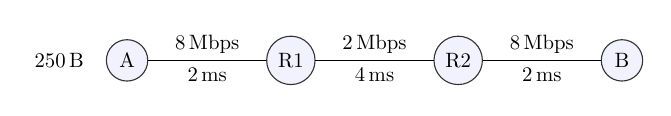
\begin{tikzpicture}[
    scale = 0.75, transform shape,
    >={Latex[black, length=1mm]},
    node distance=2cm,
    roundnode/.style={
        circle, draw=black!80, fill=blue!5, minimum size=7mm
      },
  ]
  \node[roundnode](A) {A};
  \node[roundnode](R1) [right=of A] {R1};
  \node[roundnode](R2) [right=of R1] {R2};
  \node[roundnode](B) [right=of R2] {B};
  \node[node distance=0.25cm] [left=of A] {\qty{250}{\byte}};
  \path[-]
    (A) edge [] node[above]{\qty{8}{Mbps}} (R1)
    (R1) edge [] node[above]{\qty{2}{Mbps}} (R2)
    (R2) edge [] node[above]{\qty{8}{Mbps}} (B)
    (A) edge [] node[below]{\qty{2}{ms}} (R1)
    (R1) edge [] node[below]{\qty{4}{ms}} (R2)
    (R2) edge [] node[below]{\qty{2}{ms}} (B)
  ;
  \end{tikzpicture}
  \begin{scriptsize}
    \begin{itemize}[itemsep=0em]
      \item sending 4 packets from A to B
      \item In diagram propagation dealay is below link, and speed is above.
      \item base output delay is the transmission delay $\frac{\ell_\text{\tiny{pkt}}}{S_\text{\tiny{link}}}$ (use same units)
      \item base input delay is just the propagation delay.
    \end{itemize}
  \end{scriptsize}
  \resizebox{8cm}{!}{
    \begin{tabular}{ |r|r|r|r|r|r|r| }
      \hline
      \multicolumn{1}{|c|}{\textbf{src}} & \multicolumn{1}{c|}{speed} & \multicolumn{1}{c|}{prop} & \multicolumn{1}{c|}{speed} & \multicolumn{1}{c|}{prop} & \multicolumn{1}{c|}{speed} & \multicolumn{1}{c|}{prop} \\
      \hline
      \textbf{base} & 0.25ms & 2.00ms & 1.00ms & 4.00ms & 0.25ms & 2.00ms \\
      \hline
      \hline
      \multicolumn{1}{|c|}{P$_{\#}$} & \multicolumn{1}{c|}{A$\to$} & \multicolumn{1}{c|}{$\to$R1} & \multicolumn{1}{c|}{R1$\to$} & \multicolumn{1}{c|}{$\to$R2} & \multicolumn{1}{c|}{R2$\to$} & \multicolumn{1}{c|}{$\to$B} \\ [0.6ex]
      \hline
      1 & 0.25ms & 2.25ms & 3.25ms & 7.25ms & 7.50ms & 9.50ms \\
      \hline
      2 & 0.50ms & 2.50ms & 4.25ms & 8.25ms & 8.50ms & 10.50ms \\
      \hline
      3 & 0.75ms & 2.75ms & 5.25ms & 9.25ms & 9.50ms & 11.50ms \\
      \hline
      4 & 1.00ms & 3.00ms & 6.25ms & 10.25ms & 10.50ms & 12.50ms \\
      \hline
    \end{tabular}
  }
\end{center}
First fill the entire table using the base delay for each column. Now
modify the table left to right and top to bottom without skipping
columns. For every output column ($X\to$) take each term and add to it
the max of the terms to the left and above (use 0 if there is none). Then
for every input column ($\to X$) simply add to each term the value of
the column to the left.
\subsection{The Big Picture}
\begin{center}
  \resizebox{8cm}{!}{
  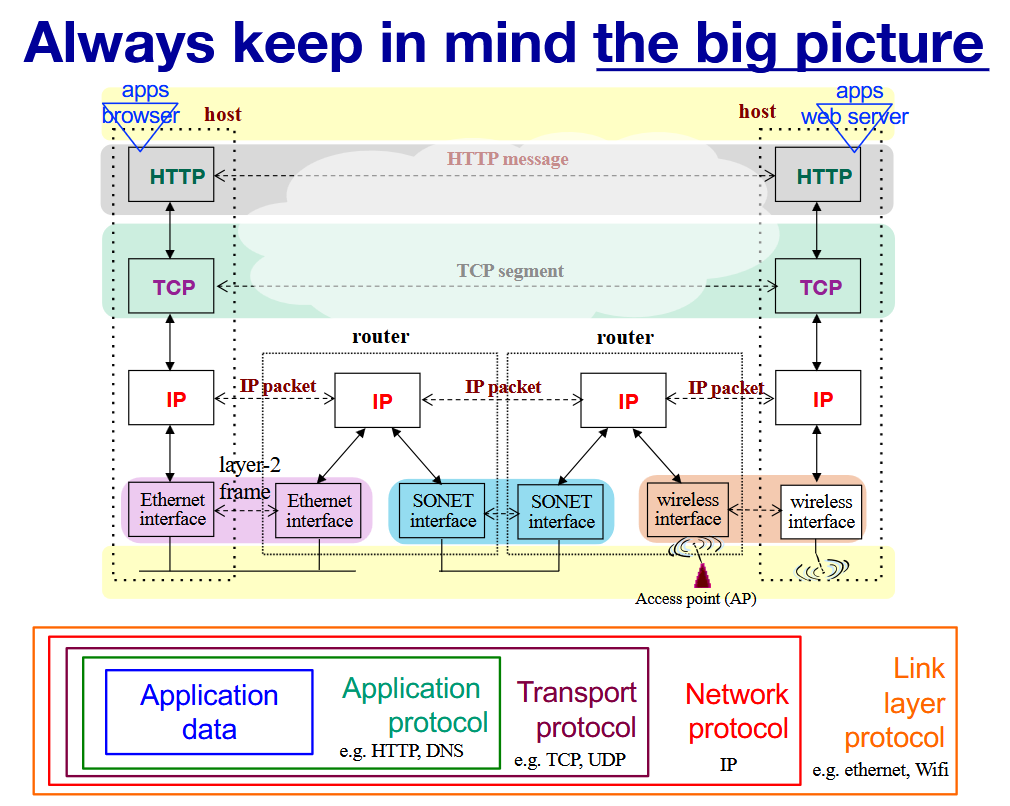
\includegraphics[]{images/big-picture.png}
  }
\end{center}
\subsection{IP Tunneling}
\begin{center}
  \resizebox{8cm}{!}{
  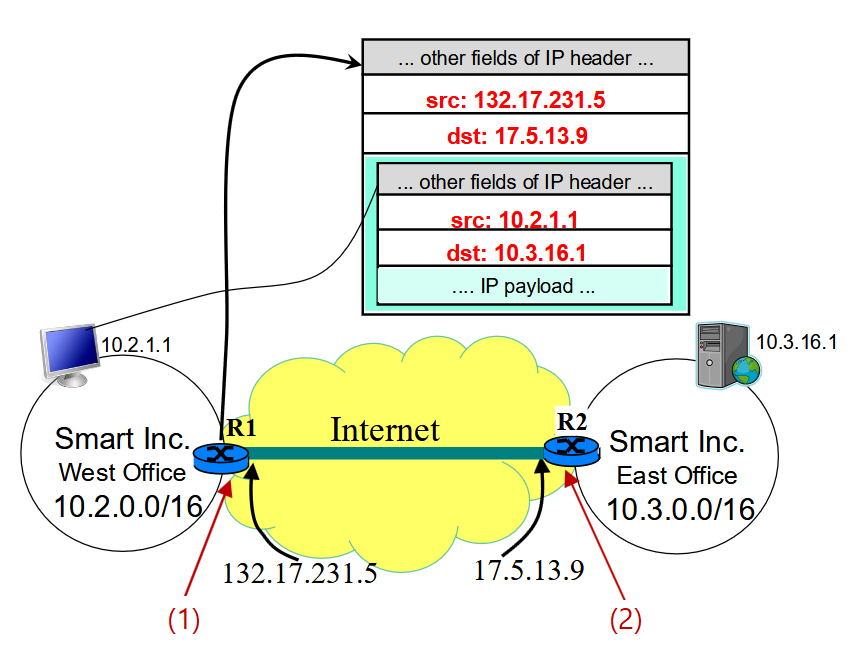
\includegraphics[]{images/ip-in-ip.png}
  }
\end{center}
(1) This NAT router knows the Smart Inc. East Office’s (private) address
block and its NAT router’s public IP address (the same is true for R2).

(2) When an IP node receives an IP packet and see the destination is its
own address, it removes the outer most header and look into next header.
\subsection{MTU Frag Example}
\begin{center}
  \resizebox{8cm}{!}{
  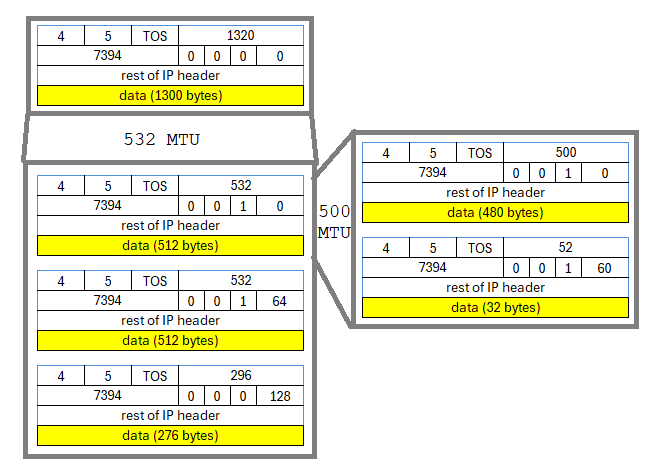
\includegraphics[]{images/mtu-frag-example.png}
  }
\end{center}
\subsection{DHCP Discovery}
\begin{center}
  \resizebox{8cm}{!}{
  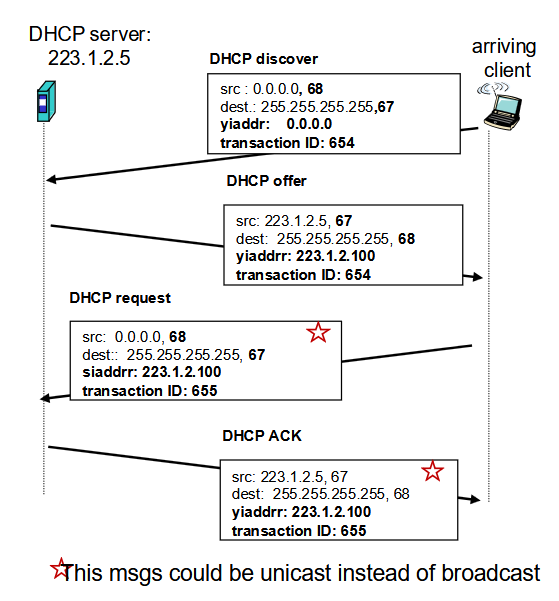
\includegraphics[]{images/dhcp-discovery.png}
  }
\end{center}
\subsection{TSL exchange diagram}
\begin{center}
  \resizebox{8cm}{!}{
  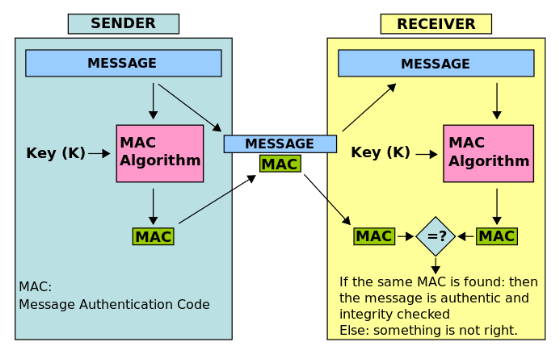
\includegraphics[]{images/tls-mac-diagram.png}
  }
\end{center}
\subsection{AS No Valley}
\begin{center}
  \resizebox{8cm}{!}{
  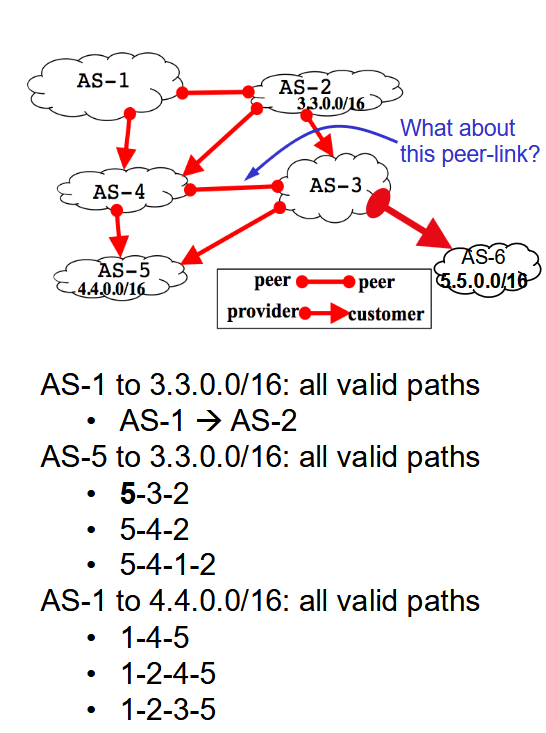
\includegraphics[]{images/as-no-valley.png}
  }
\end{center}
\subsection{Efficiency of Slotted Aloha}
\begin{center}
  \resizebox{8cm}{!}{
  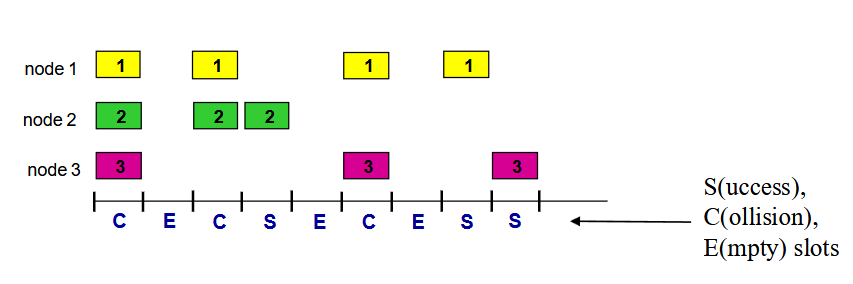
\includegraphics[]{images/aloha-detail.png}
  }
\end{center}
\begin{center}
  \resizebox{8cm}{!}{
  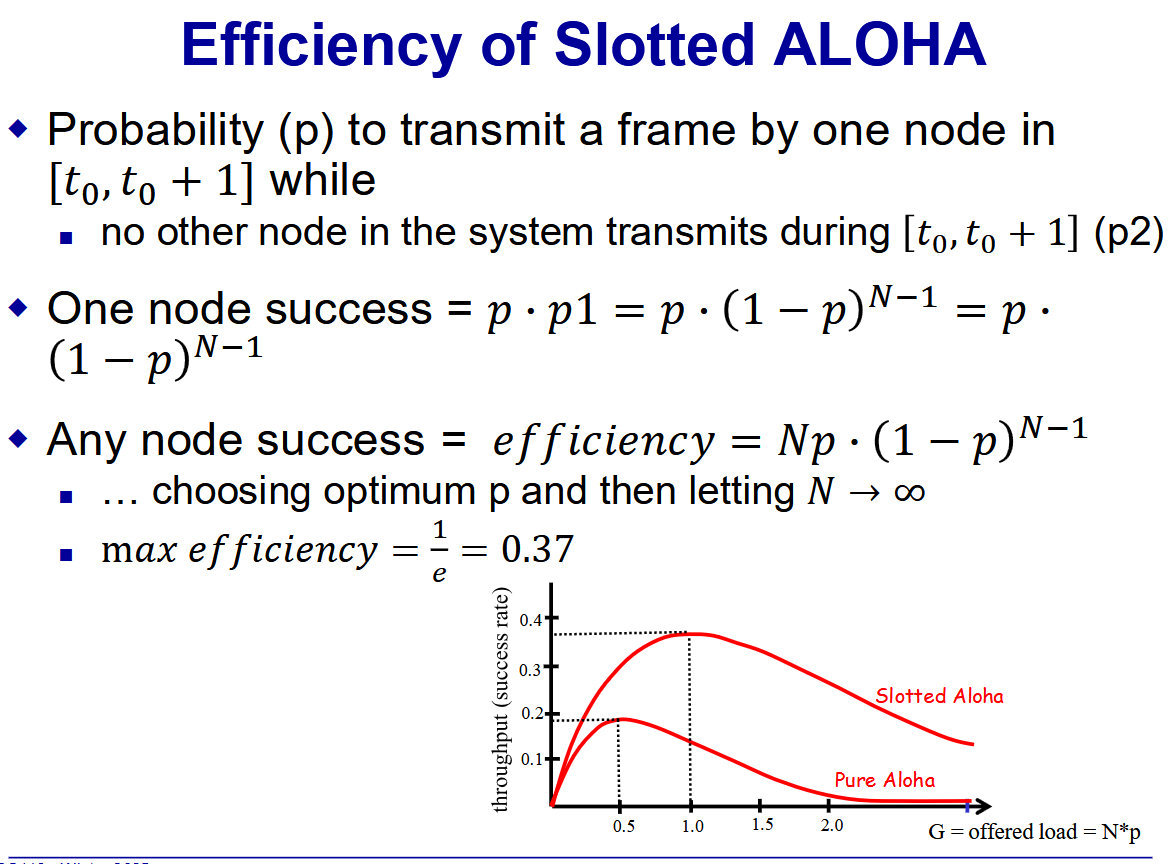
\includegraphics[]{images/eff-aloha.png}
  }
\end{center}
\subsection{Efficiency of Slotted Aloha} \label(ssec:bytestuffing)
\begin{center}
  \resizebox{8cm}{!}{
  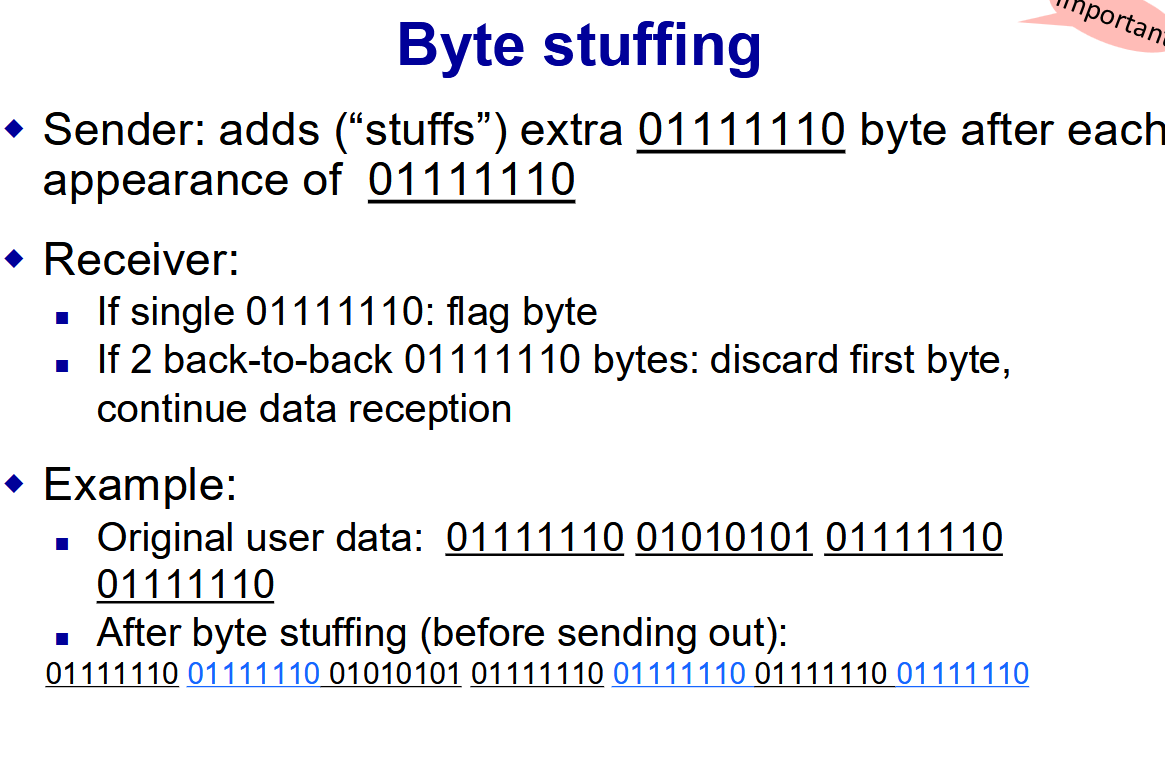
\includegraphics[]{images/byte-stuffing.png}
  }
\end{center}
\subsection{Efficiency of Slotted Aloha} \label(ssec:bytestuffing)
\begin{center}
  \resizebox{8cm}{!}{
  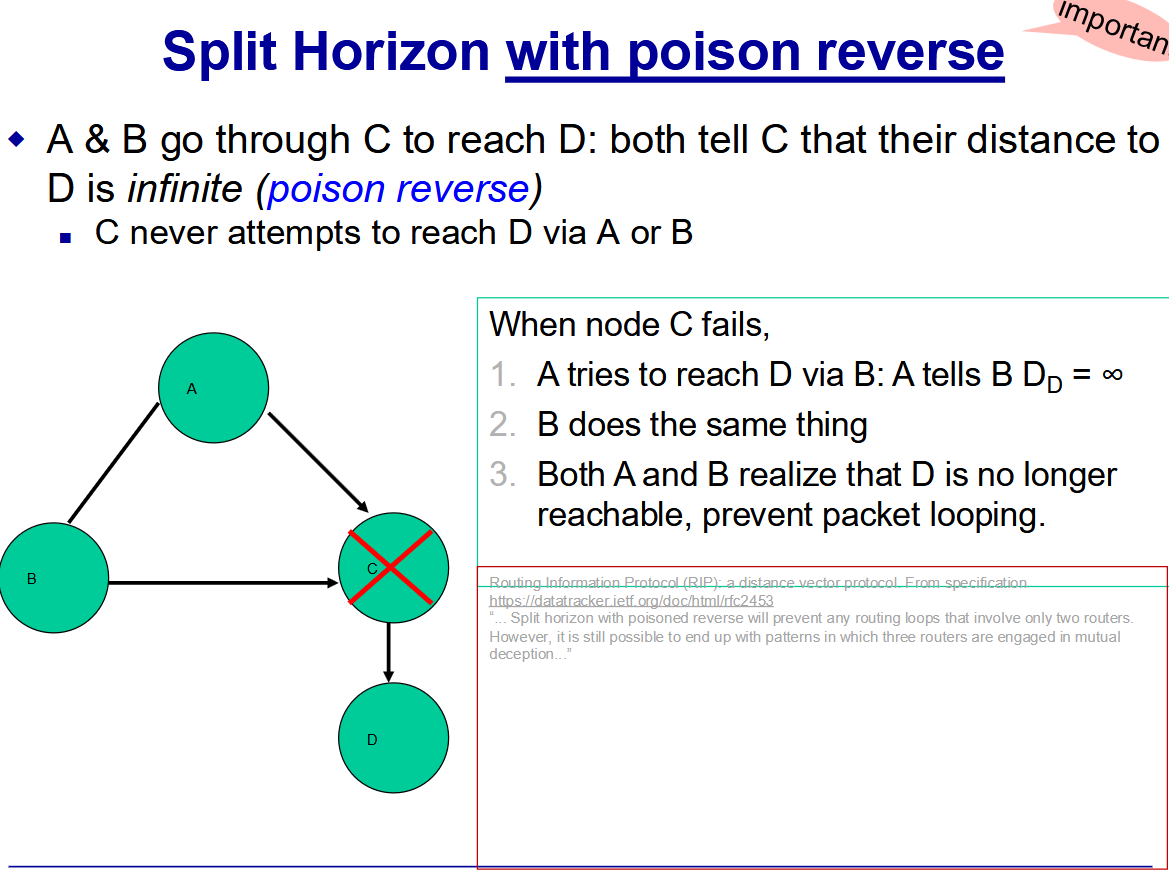
\includegraphics[]{images/split-poison.png}
  }
\end{center}
\end{multicols*}
\end{document}